\section{Test-bed Environment and Experiments}
\label{sec:evaluation}

The web application's testing strategy involved a blend of manual testing in the Integrated Development Environment (IDE) and using Postman for HTTP request evaluations. This approach aimed to ensure the application's reliability and functionality.

\subsection{Testing With Postman}

For backend validation, Postman was the tool of choice. It helped test HTTP requests, ensuring backend stability before integration with the frontend. The process began by identifying the types of requests the frontend would make, including those for polls, results, users, and votes. These requests were defined and executed in Postman, allowing for the observation and verification of output in JSON format. This approach resulted in a set of repeatable tests to continually verify backend performance, especially when modifications were made.

\begin{figure}[!htbp]
    \centering
    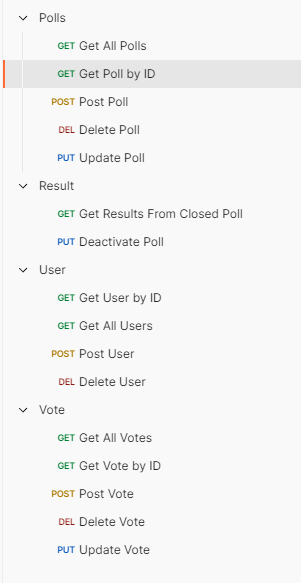
\includegraphics[width=0.3\linewidth]{figs/PostmanRequests.png}
    \caption{List of Postman requests}
    \label{fig:PostReq}
\end{figure}

Initially, our focus was to determine the range of requests that the front end of the application would execute. This investigation culminated in the identification of a series of key requests, specifically targeting Polls, Results, Users, and Votes. This comprehensive list of requests is illustrated in Figure 4, providing a clear overview of the interactions expected between the front end and the back end of our system.

\begin{figure}[!htbp]
    \centering
    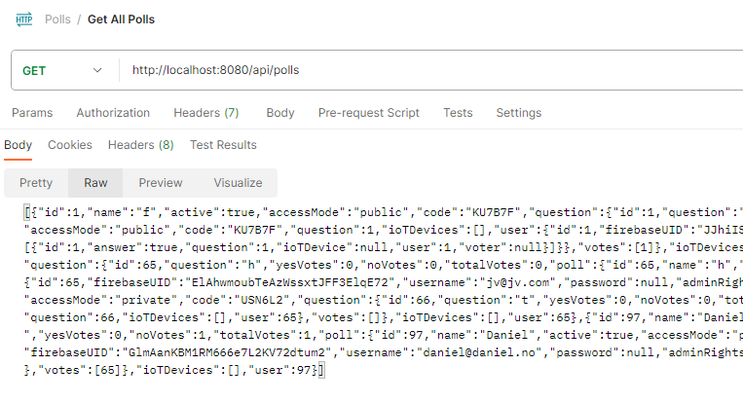
\includegraphics[width=0.5\linewidth]{figs/PostmanGetAllPolls.png}
    \caption{The request for all Polls in Postman}
    \label{fig:PostAllPolls}
\end{figure}

\begin{figure}[!htbp]
    \centering
    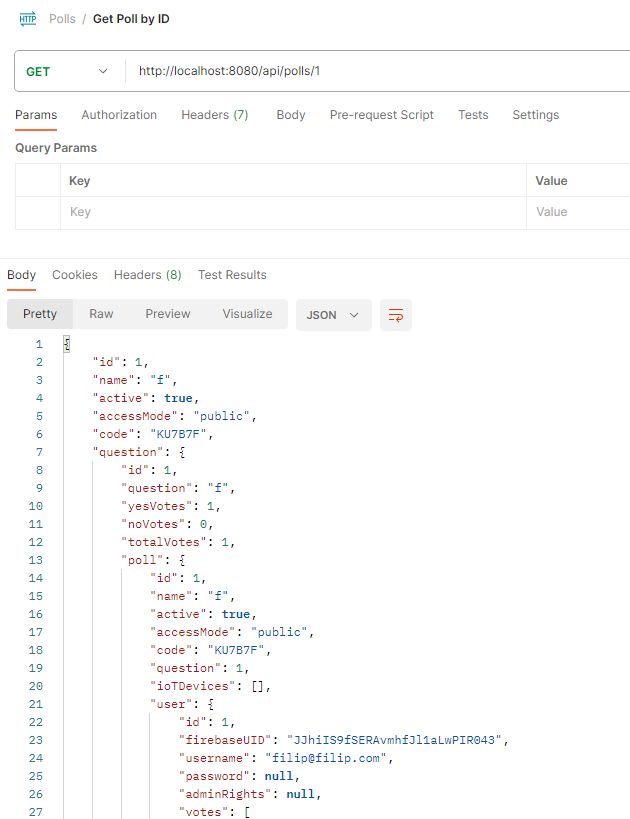
\includegraphics[width=0.5\linewidth]{figs/PostmanGetPollById.png}
    \caption{Request for a specific Poll by ID, and the resulting JSON}
    \label{fig:PostPollById}
\end{figure}

Subsequently, these identified requests were meticulously formulated and executed to monitor their respective outputs, which were primarily in JSON format. This process is exemplified in Figure 5 and Figure 6, showcasing the outcomes of different requests. The execution of these requests not only allowed for real-time observation of system responses but also led to the creation of a suite of tests. These tests could be readily deployed to evaluate the backend's functionality at any given time. This approach ensured a robustly tested and verified backend, establishing a solid foundation prior to initiating the development of the frontend.

\subsection{IDE-Based Manual Testing}

With the backend nearly complete and validated, frontend testing was conducted by running the application in the IDE. This involved using the web page to assess functionality and utilizing the IDE's debugger for in-depth testing. Regular checks and console printing were integral to this process.

\subsection{Testing Experience}

Overall, the testing experience was highly effective. Testing the backend with Postman before moving to the frontend streamlined the integration process, reducing the need for extensive backend revisions. The saved Postman requests also facilitated periodic retesting, ensuring continued backend integrity.

Frontend testing was also successful, with new features being checked alongside existing ones to maintain overall functionality. However, this manual approach to testing may become cumbersome as the application scales, indicating a potential need for automated testing in future development phases.

Regular presentations required us to thoroughly test all the old and new parts of our project, so everything ran smoothly when we showed it off. This approach really highlighted how important it is to keep testing our work carefully and consistently as we develop it.